\chapter{Clustering algorithms in high energy physics}
\label{ch:1}
\section{The clustering problem}
\label{ch:clustering_problem}
Cluster analysis is, in general, a non trivial problem. Even the definition of cluster can change wildly depending on the context. Due to these circumstances, many clustering methods have been developed, based on various notions of cluster~\cite{clustering}. Currently, some of the most common clustering algorithms can be divided in the following categories: 
\begin{itemize}
    \item \textit{Connectivity models}: generally based on distance between points;
    \item \textit{Partitioning}: such as k-mean algorithms, represent each cluster by optimizing a single function which depends on the distance~\cite{k-mean};
    \item \textit{Density models}: consider dense regions in the data space as clusters;
    \item \textit{Hierarchical methods}: build clusters following a recurring dendrogram with splitting or merging.
\end{itemize}
There is no general correct way to produce clusters: each problem requires a specific approach depending on the conditions known a priori, the expected results and also the desired performance.

In the upgrade plan for the future revision of LHC, HL-LHC (High Luminosity Large Hadron Collider), calorimeters with high readout granularity have been suggested to observe fine grained images of hadronic and electromagnetic showers~\cite{high_granularity}. In the case of CMS, the High Granularity calorimeter (HGCAL) will replace the current endcap calorimeters. It consists of several layers and has both an electromagnetic and hadronic compartments.
\begin{itemize}
    \item The Electromagnetic section (CE-E) is made up of cassettes each containing two layers of sensors and two layers of absorber;
    \item The Hadronic section (CE-H) contains both silicon sensors and scintillator tiles, as shown in Figure~\ref{fig:hgcal_sensors}. 
\end{itemize}
The latter is divided into two sections: the first having a finer sampling than the second. The first few layers of the fine part of the Hadronic section are made of hexagonal silicon sensors only, each having a surface area of 0.5 or 1 cm$^2$; layers in the last part of the hadronic compartment instead are mixed, with both silicon sensors and scintillator tiles~\cite{hgcal}.

\begin{figure}[H]
    \centering
    \begin{subfigure}[t]{0.3\textwidth}
    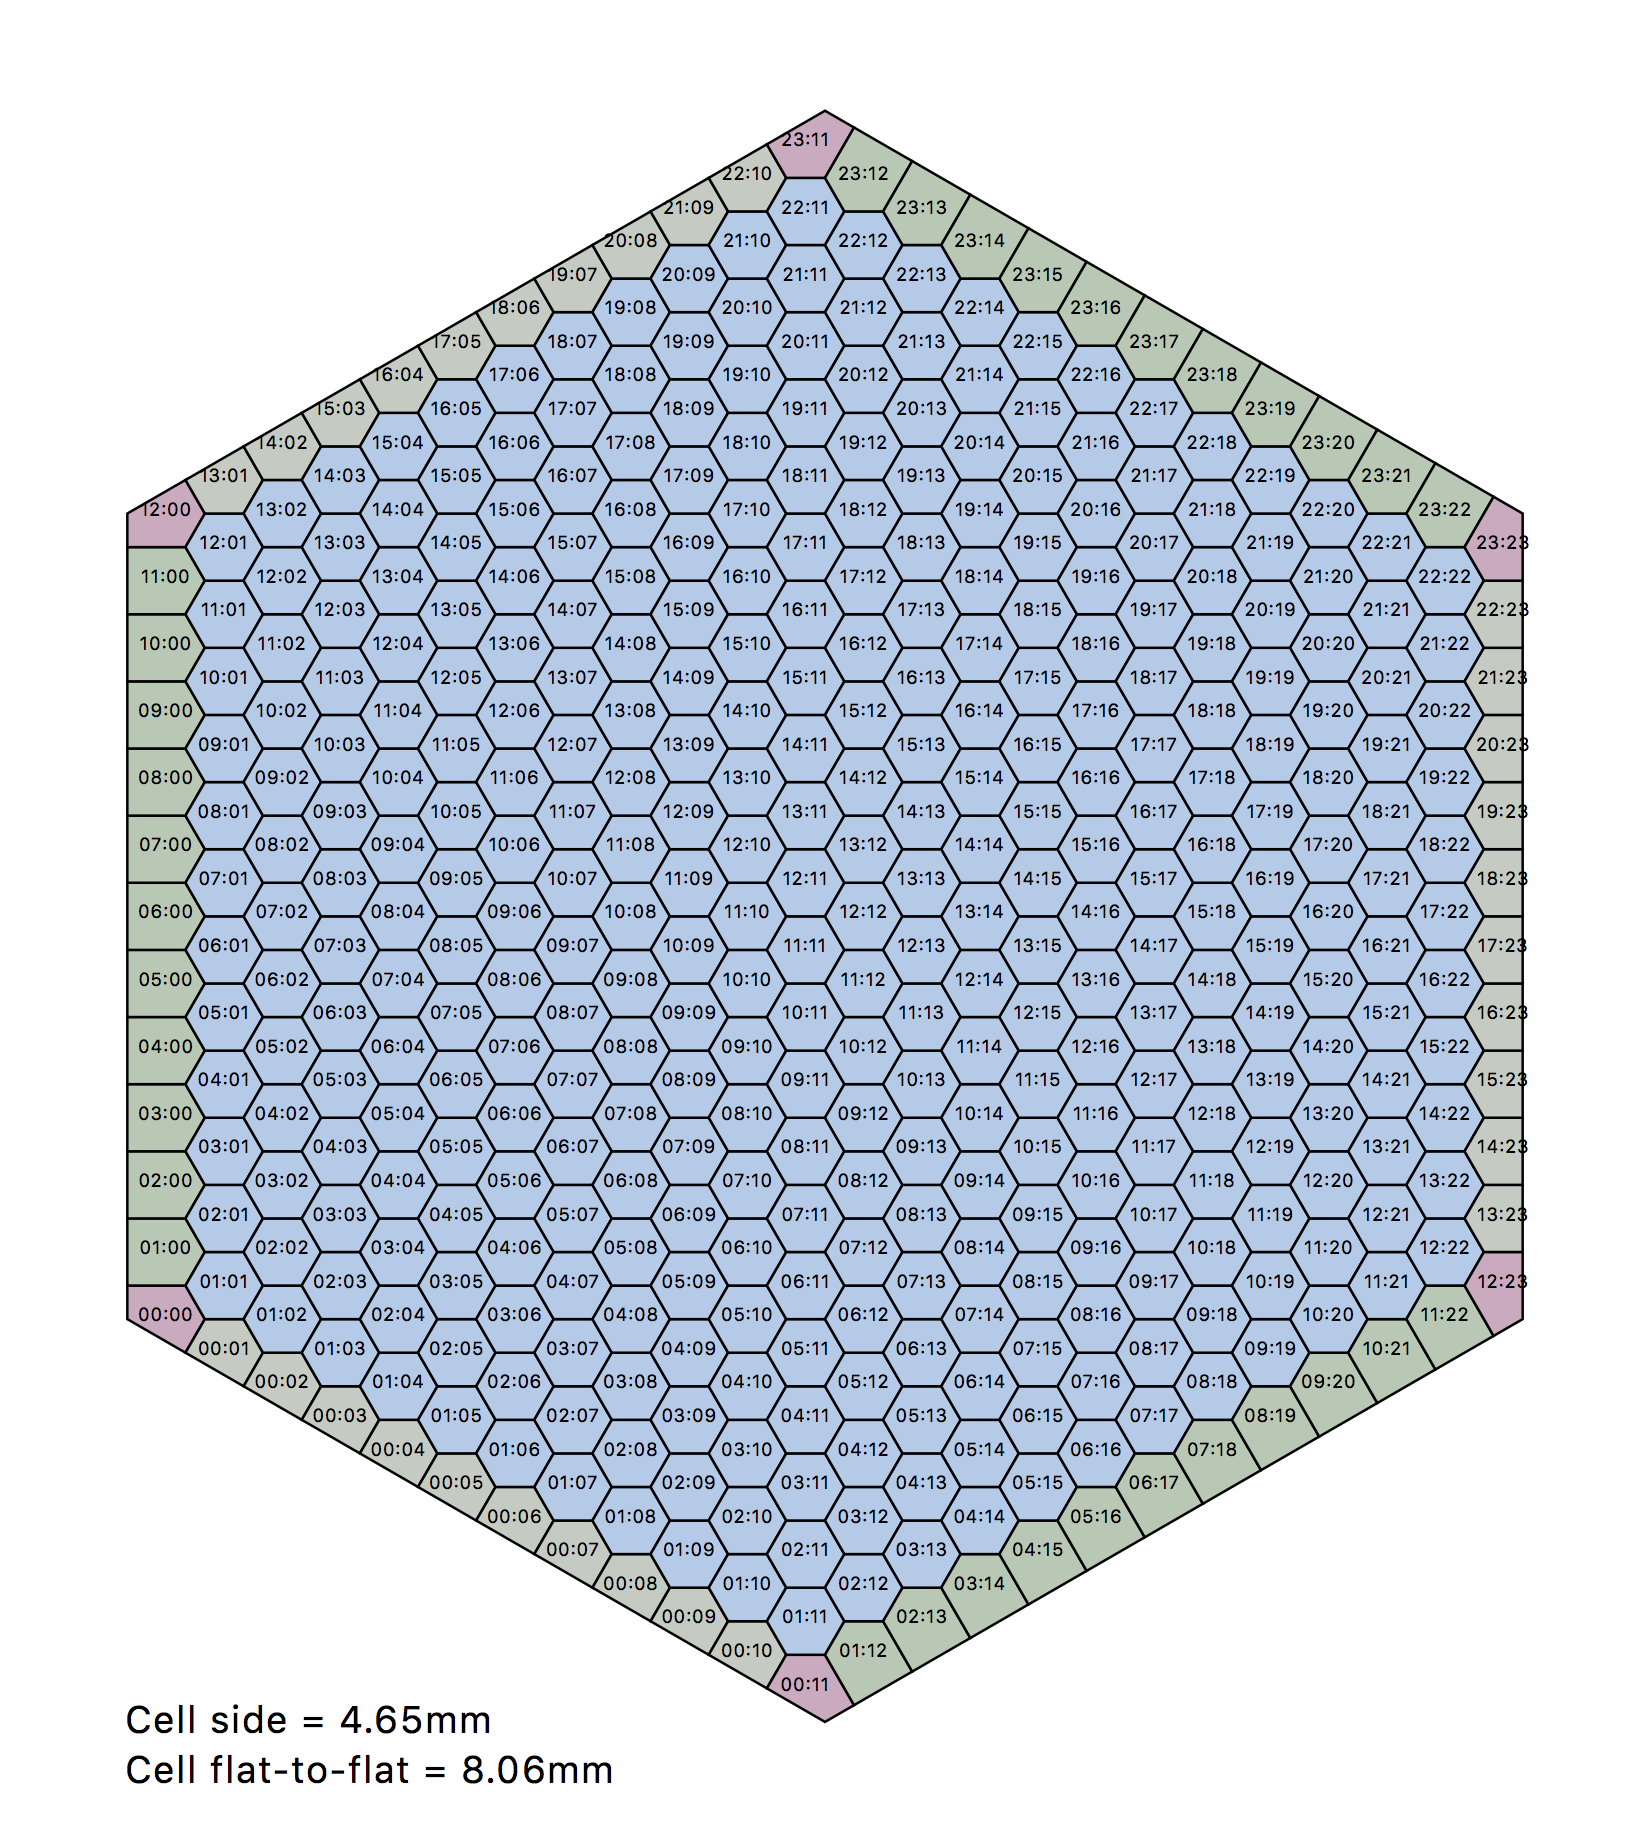
\includegraphics[width=\textwidth]{media/high_density_cells.png}
    \caption{High density silicon \\ sensors}
    \end{subfigure}
    \begin{subfigure}[t]{0.3\textwidth}
    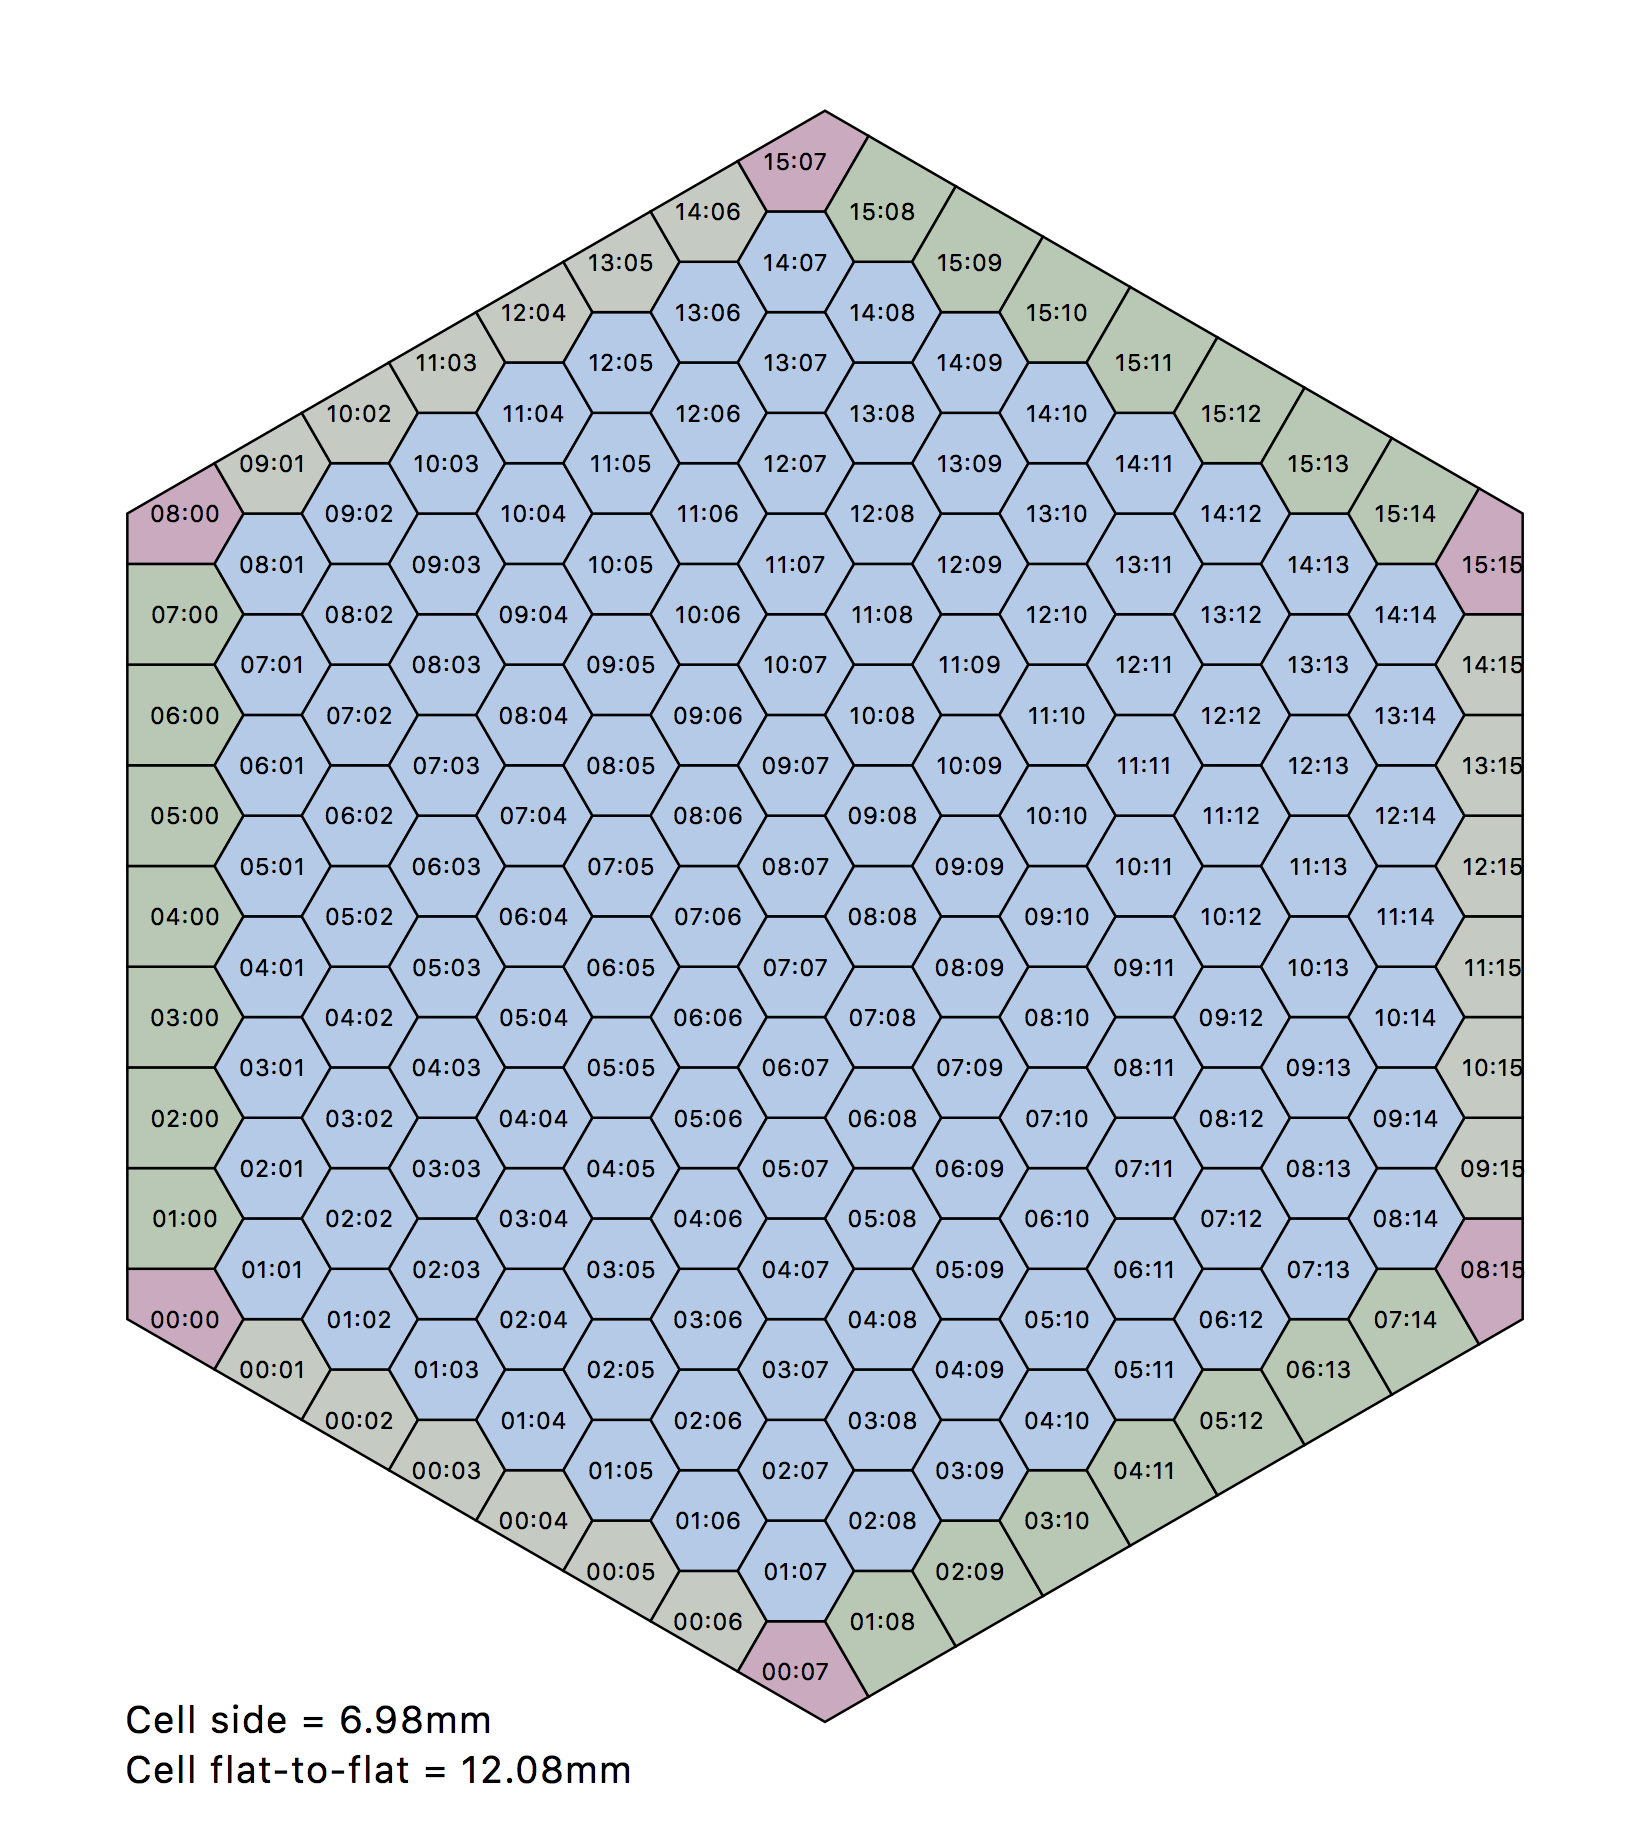
\includegraphics[width=\textwidth]{media/low_density_cells.png}
    \caption{Low density silicon \\ sensors}
    \end{subfigure}
     \begin{subfigure}[t]{0.3\textwidth}
     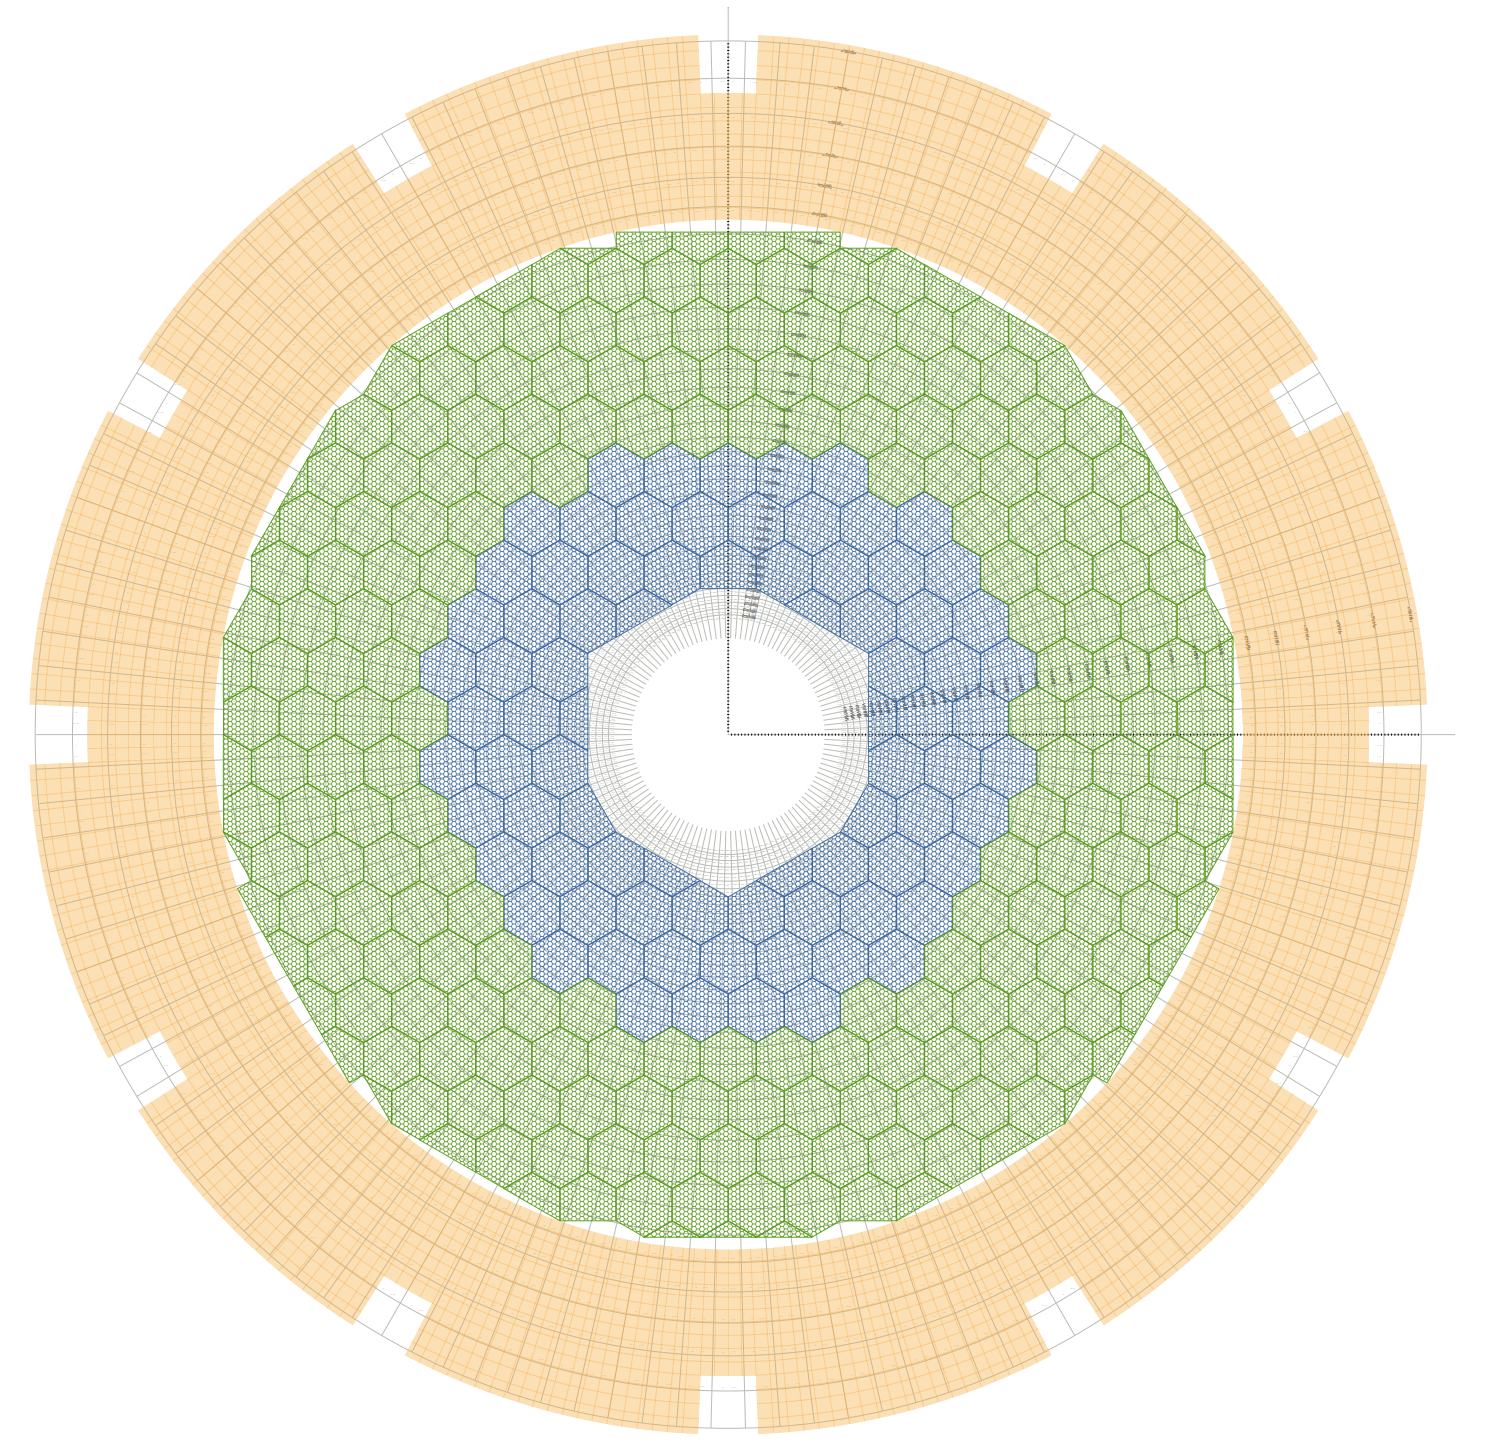
\includegraphics[width=\textwidth]{media/mixed_layer.png}
    \caption{Layout of a mixed layer with both silicon and scintillator sensors}
    \end{subfigure}
    \caption{Schematic representation of the different sensor layouts on HGCAL layers.}
    \label{fig:hgcal_sensors}
    \source{\emph{:}\cite[slide 4]{HGCAL_layers}}
\end{figure}

Following a collision, particles that enter the detector interact with its materials and produce showers, whose energy is measured by the sensors on each layer. By clustering the resulting energy deposits (hits) it is possible to reconstruct the shower shape and its main parameters and, after other steps in the reconstruction, identify all of the hits produced by a single particle. Since the calorimeter will have an unprecedentedly high granularity, the most efficient way to cluster the deposits is to group them in bidimensional clusters layer by layer~\cite{2d} and then connect clusters in subsequent layers with pattern recognition algorithms. In this context, a computational challenge arises, due to the larger amount of data collected in the era of HL-LHC and the limited computational time available at the CMS High Level Trigger (HLT)~\cite{high_level_trigger}, responsible for the selection of the events of interest. Since event reconstruction must happen at millisecond-level time frames, the algorithm employed needs to be highly efficient and scale well (i.e. linearly or better) as the number of hits increases, in order not to be a bottleneck for the performance. These specific requirements have brought CMS to explore the potential of heterogeneous computing with hardware accelerators such as Graphics Processing Units (GPUs) or FPGAs which can help achieving a higher number of events processed per unit time (throughput) and better energy efficiency. 

The input of any clustering algorithm is a set of $n$ points and the output is a set of $k$ clusters which is usually one or two orders of magnitude smaller than $n$. For clustering in high energy physics, $n$ usually varies from a few thousands to a few millions, while k generally depends on the number of incoming particles as well as the number of layers of the calorimeter. In the case of the HGCAL detector, the average number of hits in a cluster $m=n/k$ can be estimated to be in the order of $10$. This leads to the relation between the number of hits $n$, the number of clusters $k$ and the average number of hits in a cluster $m$ as $n > k \gg m$. 
Starting from partitioning algorithms, these are not applicable in this case since the number of clusters $k$ is not known a priori. Moving to hierarchical clustering, this method is not suitable as well, since it does not scale well with the number of points as each decision to split or merge needs to scan over many objects or clusters. Density based methods are the most interesting for the HGCAL application, as they are capable of finding clusters of any shape and are efficient for large spacial data collections. However, well-known existing density-based clustering algorithms intrinsically include serial processes that are hard to parallelize. Due to all these reasons, CMS has developed its own clustering algorithm to fit the specific application in the HGCAL detector.

\section{CLUE standalone}
\subsection{What is CLUE?}
\label{ch:clue}
Clustering of Energy (CLUE) is ``a fast parallel clustering algorithm for high granularity calorimeters in high-energy physics"~\cite{CLUE}, which was specifically developed to address all of the aforementioned challenges. This algorithm follows a density-based approach with some specific optimizations implemented to give it a greater expression of parallelism. The input data of the algorithm is a series of hits each having its corresponding coordinates ($x$, $y$ and $layer$) and $energy$. For each point, two key variables are calculated: the local density $\rho$ and the separation $\delta$. The first one represents the energy density in the area of the hit, while the second variable corresponds to the distance from the hit and the nearest hit with higher local density. From these two parameters it is possible to cluster points depending on arbitrary thresholds set on a case-by-case basis. 

\subsection{Clustering procedure}
\label{ch:clustering_procedure}
Since CLUE was specifically designed to be used in high-energy calorimetry, where hits are registered on sensor cells whose layout is a multi-layer tessellation, the algorithm's data is indexed with a fixed grid, which divides the space into rectangular bins. This indexing choice allows to fast query the neighborhood of multiple points at the same time to better express parallelism on GPUs and when running on multiple threads.

CLUE requires three parameters: the critical distance, $d_c$, is the cut-off distance used for the calculation of the local density; the critical density, $\rho_c$, is the minimum local density to promote a point as a seed or the maximum density to demote it as an outlier; finally the outlier delta factor, $odf$, is a multiplicative constant applied to the critical distance to obtain the maximum distance between a point and its nearest point with higher density over which the point is excluded from the clustering process. These parameters are chosen at runtime and can be tuned by the user based on the clustering application. For example, $d_c$ can be tied to the expected shower size and the granularity of the detectors (possibly differing between silicon-based layers and scintillators), $\rho_c$ can be tuned to maximize the signal to noise ratio and $odf$ can be chosen considering the shower separation. In this way, the use of configurable parameters allows CLUE to be more flexible at clustering different events for the specific desired goals of physics. 

\begin{figure}[tb]
    \centering
    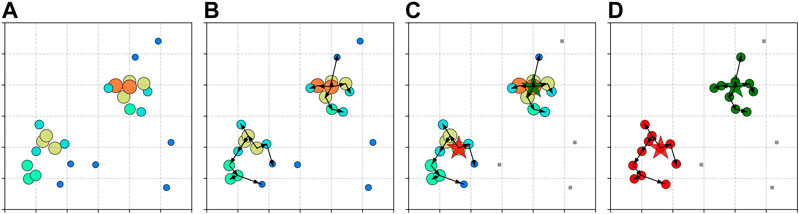
\includegraphics[width=\textwidth]{media/clustering_procedure.jpg}
    \caption{Schematic representation of CLUE clustering procedure: from fixed spacial grid to clusters.}%~\cite{CLUE}.}
    \source{\emph{:}~\cite{CLUE}, figure 2}
    \label{fig:clustering_procedure}
\end{figure}

In Figure~\ref{fig:clustering_procedure} the clustering procedure of CLUE is shown in a $6\times6$ grid. First, a fixed grid is constructed and each point is arranged in the bin mapped to its coordinates. Then, CLUE calculates the local density $\rho$ for each point by querying its neighborhood, as shown by the different sized and colored dots (A). Afterwards, each point gets assigned a nearest higher $nh$, defined as the nearest point with higher local density and their distance $\delta$ is calculated (B). Points with $\rho$ higher than the critical density $\rho_c$ and $\delta$ greater the critical distance $d_c$ are promoted as seeds, while points with lower density and larger separation ($\delta > d_c \times odf$) are demoted to outliers. All the other points that are neither seeds nor outliers are marked as followers of their respective nearest highers. As a consequence of this logic, each seed has a chain of followers which can be iteratively navigated to build a cluster. At the end of the procedure, only clusters and outliers remain, with the latter points having no followers and not being followers of any other point.

\subsection{GPU implementation}
\label{ch:gpu_impl}
As previously discussed, CLUE was first developed in order to provide a parallelizable clustering algorithm for high occupancy scenarios in high energy physics, targeting GPUs as hardware accelerators.  The main advantage of this class of devices is given by their massive number of physical threads, than can be used to make computations in parallel. 
The GPU implementation of the CLUE algorithm takes advantage of the multi-threading capabilities of GPUs thanks to the used data structure and the design of each function in the step-by-step procedure. It assigns one GPU thread to each point, for a total of $n$ threads, to create the spacial grid, calculate the local density and separation, promote or demote the point and register points as followers of the corresponding nearest higher. In the last step of the algorithm, each seed is assigned to a single thread, with a total of $k$ threads that build clusters in parallel going through the chain of followers iteratively. Since the results of each step are required in the following ones, it is necessary to synchronize all the threads before moving onto the next computation. This is naturally done by implementing each step into a separate kernel. Data for all of the points is stored in the global device memory as a single structure-of-array (SoA), which contains the points' coordinates, layer numbers and energies.

One key factor to take into account when developing software for GPUs is that, due to the parallel nature of the execution, it can happen that multiple threads try to access and modify the same address in global memory at the same time. For the CLUE application, thread conflicts can happen in three cases:
\begin{enumerate}
    \item multiple points need to register to the same bin simultaneously;
    \item multiple points need to register to the list of seeds simultaneously;
    \item multiple points need to register as followers to the same point simultaneously.
\end{enumerate}
Because of this, some atomic operations are required to avoid race condition among threads. When performing an atomic operation, a thread is granted exclusive access to a specific memory location that becomes inaccessible to all other threads until it finishes. The usage of atomic operations naturally causes some serialization among threads in a race. Its impact is negligible in cases 1 and 3, since the bin dimension and the number of followers per point are usually small. By contrast, serialization in case 2 can cause a significant slowdown since the number of seeds $k$ can be large. However, this operation is still faster on GPU memory when compared to the data transfer between host and device; therefore, the total execution time of CLUE does not suffer significantly from this serialization.

\section[Heterogeneous computing and compatibility layers]{Heterogeneous computing and compatibility \\ layers}
\label{ch:heterogeneous_compatibility}

\subsection{The need for heterogeneous computing}
\label{ch:heterogeneous}
The high luminosity upgrade for the LHC, scheduled before the beginning of the next runs from 2029 onwards, will increase the number of collisions per unit time (namely the \textit{luminosity}) by roughly a factor of 10, resulting in an average \textit{pileup} of 200 proton-proton collisions every $25~ns$. Such an increase in the number of events per second will pose an incredible challenge for both online and offline software reconstruction of each experiment~\cite{high_luminosity}. This added complexity far exceeds the expected increase in the processing power for conventional CPUs and thus calls for the exploration of novel and different solutions. One such possibility is \textit{heterogeneous computing}, which is already being exploited by industry and high performance computing centers to achieve better efficiency and higher throughput by matching the job to the best possible architecture. Specifically, applying this new paradigm to CMS software reconstruction (CMSSW) and its framework means that part of the work can be offloaded to one or more graphics processing units (GPUs), thus easing the load on the CPUs while simultaneously increasing the total throughput and improving energy efficiency. Tasks offloaded to a GPU are executed in a parallel fashion and, most importantly, asynchronously with respect to the code running on CPU, meaning that the CPU resources freed by offloading work to GPUs can be used for other tasks at the same time. The shift to heterogeneous computing has already proved to be a success for CMS offline reconstruction, where GPU implementations show up to three times increase in performance in some cases~\cite{high_luminosity}. However, adopting heterogeneous computing also poses some challenges, especially in code portability and maintainability. While having the possibility to offload work on different hardware looks promising, it also means that in order to be able to efficiently execute software on heterogeneous hardware, the code should be written and optimized for each specific backend\footnote{In software engineering, the physical infrastructure or hardware on which the code is executed.} to be targeted. Even considering only the main GPU manufacturers, one would need to take into account three different implementations for each kernel in all of the algorithms, leading to a massive code duplication, whose maintenance represents an insurmountable challenge and a great resource sink. 

These reasons led to explore different compatibility layers to ease the transition to heterogeneous computing. A candidate layer must support multiple architectures such that the programmer can write a single source code without having to sacrifice performance. 

\subsection{The Patatrack group}
The adoption of heterogeneous computing in CMSSW has been first proposed by the CMS Patatrack group. The group was founded in 2016 and is composed by a diverse set of people whose main objective is to demonstrate that it is possible to adopt heterogeneous computing in both online and offline reconstruction with benefits both in terms of software and hardware. Firstly, the team developed parallelizable algorithms for calorimetry reconstruction as well as the Pixel Detector\cite{pixeltrack}, with promising results which led to a wider push to support heterogeneous computing in CMMSW. In 2021, the group managed for the first to reconstruct collisions with GPUs\cite{HLT_GPUs} offloading $\sim$30\% of the HLT processing to GPUs. The number of algorithms that can run on GPUs is planned to grow during subsequent runs with the goal of offloading at least $\sim$50\% of the processing during Run-4 of HL-LHC and $\sim$80\% in Run-5. In this context, the team is developing new algorithms as well as porting old ones to GPUs.The work presented here is part of Patatrack's research on compatibility layers for heterogeneous computing and development of parallelizable algorithms.

\subsection{SYCL and other compatibility layers}
As previously discussed, the adoption of heterogeneous computing, while improving performance and efficiency, also poses a great challenge in the ability to maintain code and port it to different architectures. Therefore, in recent years the development of portability layers has ramped up significantly as more and more applications require to offload work to different accelerators. Many different solutions are now available, each proposing a different way to handle the problem but all trying to use a single source code to produce a unique executable file able to run on as many different backends as possible. In this context, the CMS collaboration and in particular the High Level Trigger developers have started looking for a suitable compatibility layer to adopt for heterogeneous event reconstruction code. A large fraction of CMSSW algorithms has been successfully ported to CUDA a few years ago, and it is being executed already on both CPUs and NVIDIA GPUs (which handle the more computing-intensive parts). In order to adapt the software reconstruction to more vendors and accelerators, a large fraction of the framework has already been ported to such a compatibility layer and this new version is scheduled to run in production after the LHC Christmas shutdown between 2022 and 2023. The compatibility layer currently in use is alpaka: a header-only abstraction library for accelerator development~\cite{alpaka}. Such portability library allows the abstraction of the underling levels of parallelism by mapping some custom-defined classes to different hardware depending on the backend. In general, the work division is very similar to CUDA's grid-blocks-threads division with the addition of an extra element layer that allows for different mappings on CPUs and GPUs. In this way, the compatibility layer is able to exploit the different parallelization capabilities of each different backend. As previously stated, a large fraction of the software reconstruction has already been ported to alpaka, which thus allows to only develop and maintain one source code while still being able to run the reconstruction on both CPUs and NVIDIA GPUs. Support for other backends is still ongoing: Intel GPUs are not yet supported by alpaka itself, while AMD GPUs are officially supported, but the corresponding backend has not been implemented in the software reconstruction yet.

Although some other compatibility layers, like kokkos~\cite{kokkos}, have been explored, alpaka is, as of now, the most promising of such layers for the CMS reconstruction. However, SYCL is still a solution being tested for three main reasons:
\begin{itemize}
    \item SYCL is a royalty-free project, supported by many actors in the tech industry, which bodes well for the future support of the standard;
    \item As a new compatibility layer is developed, it is always relevant to explore its performance in comparison to native code and other compatibility layers;
    \item While not all the backends have been implemented yet, SYCL promises to support a variety of devices: from CPUs to GPUs and also Intel's FPGAs.
\end{itemize}
Furthermore, being a royalty-free project, SYCL can count on a variety of implementations which are explored in more detail in Section~\ref{ch:sycl_implementations} but, at a base level, this allows for more flexible adaptations of the standard to specific needs. 